%!TEX root = ../crimson_throne_book_main.tex
% 2015-02-22
\section{6 Erastus 4708}

With Madam Nesia in charge of the household things run a lot smoother (and cleaner) at the villa. At breakfast the companions go over their plans for the day. They want to investigate the queen's physicians, to see how far the corruption has spread.\\

They head over to the {\itshape Hospice of the Blessed Maiden} , the warehouse that was turned into the physicians' headquarters. Just as the arrive, they see a patrol with a pair of doctors leaving. Quint casts a  {\itshape detect magic} and notices that both doctors are wearing an enchanted mask. Next the heroes go inside, where they are promptly stopped at the front desk by a burly nurse. The woman is wearing leather gloves and a cloth in front of her mouth. "Get in line!" she shouts, pointing to the six sick people who are already here. A closed door behind the desk provides entry to the main hall, but a Korvosan guard blocks the way. Quint demands to see Doctor Dave Saulus, but the nurse refuses to let him through, until Sjo pulls out the Field Marshal's charter and bullies the woman into agreeing. She leads the companions through the doorway into\hyperref[fig:Hospice-of-the-blessed-maiden-515716825]{ the warehouse's vast interior which has been converted into one gigantic sick ward } . The stench of alcohol and sickness chokes each breath. Rows of stained cots cram the floor, every bed filled with its own pitiful story: men and women of all walks are groaning as the final stages of the plague consume them. The ceiling of the room is nearly 30 feet high, though a series of catwalks span the room at 20 feet. Four dark robed doctors hover amid the sick, their avian masks giving them an unnerving resemblance to crows waiting to be fed. Quint spots magic in each of the facial covers. Four Korvosan guards and one Gray Maiden walk the floor, while three more Gray Maidens patrol the catwalks above. \\

\begin{figure}[h]
	\centering
	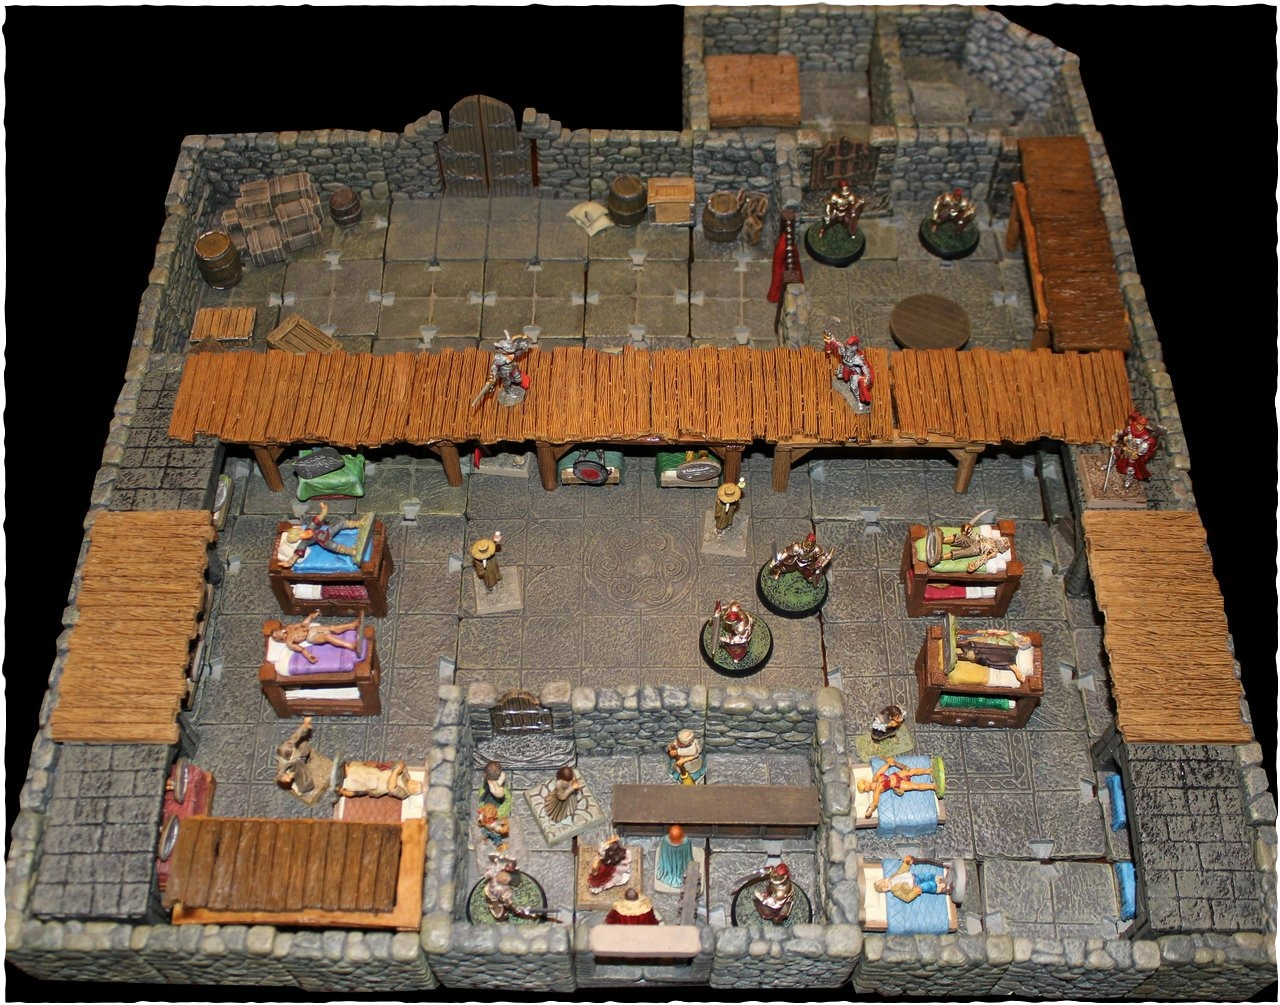
\includegraphics[width=0.4\textwidth]{images/Hospice-of-the-blessed-maiden-515716825_mod.jpg}
	\caption{Hospice of the blessed maiden}
	\label{fig:Hospice-of-the-blessed-maiden-515716825}
\end{figure}

The nurse takes the visitors to a staircase in the back and precedes them to\hyperref[fig:Hospice-of-the-blessed-maiden-upstairs-515717557]{ the fist floor } . There is a second smaller sick room upstairs, in which one of the masked doctors immediately reacts badly to the companions' arrival. Nurse Brunhilde tries to calm the man's protest and urges him to let the guests see Doctor Saulus. During this brief conversation Quint notices that the sick in here are all of Varisian stock, while the doctors are all wearing  {\itshape magic} masks again. Puk spots a leather strap bound to a patient's wrist: these poor wretches have been tied down, possibly for their own safety, but the halfling still feels bad about it. Balian gives one patient a quick look-over and is surprised to see that the man shows no signs of the plague, although he looks sedated. The ranger decides to keep quiet about it for now, but he will definitely have to inform his friends of this later. \\

\begin{figure}[h]
	\centering
	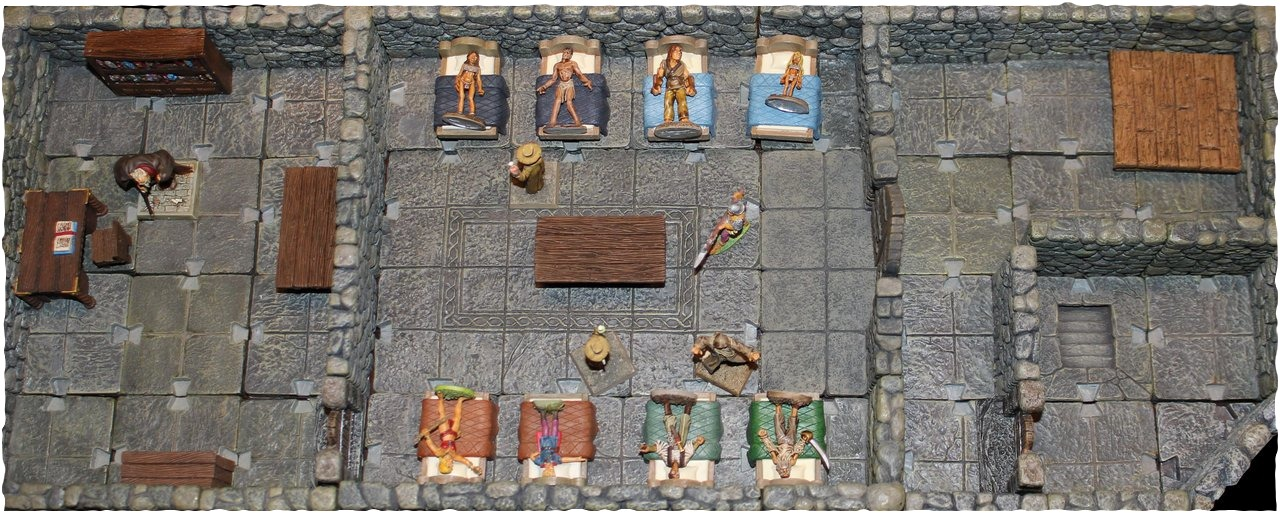
\includegraphics[width=0.4\textwidth]{images/Hospice-of-the-blessed-maiden-upstairs-515717557_mod.jpg}
	\caption{Hospice of the blessed maiden upstairs}
	\label{fig:Hospice-of-the-blessed-maiden-upstairs-515717557}
\end{figure}

Before the protesting physician can utter more objections, Sjo storms through to the back and bursts into the office of doctor Saulus. This time even\hyperref[fig:Hospice-of-the-blessed-maiden-doctor-515717926]{ the head physician is wearing an avian beak over his nose } , which again radiates magic. The companions demand that the doctor gives them an update, but the proud Chelaxian seems very displeased at their sudden arrival and is very curt in his answers. He sees no reason to give any explanation to these annoying upstarts and quickly shows them the door. Puk wants to compare the doctor's handwriting to the plague plan from Lost End and makes an attempt to snatch one of the papers on the table unnoticed. He fails miserably at it, angering the doctor even more, who has the intruders escorted out immediately. \\

\begin{figure}[h]
	\centering
	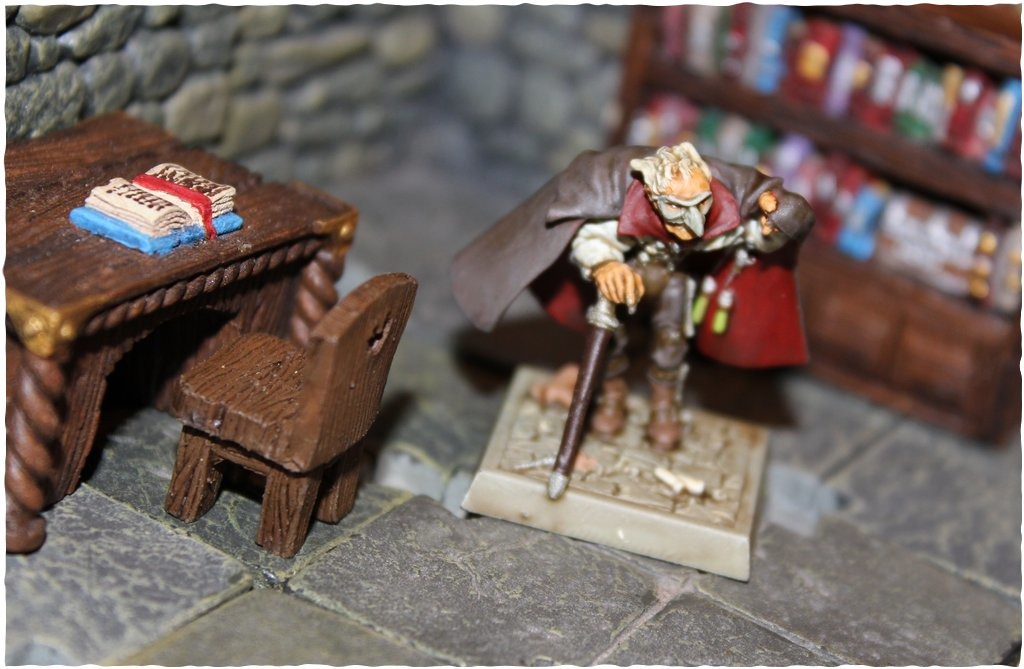
\includegraphics[width=0.4\textwidth]{images/Hospice-of-the-blessed-maiden-doctor-515717926_mod.jpg}
	\caption{Hospice of the blessed maiden doctor}
	\label{fig:Hospice-of-the-blessed-maiden-doctor-515717926}
\end{figure}

The companions contemplate what to do next: Quint wants to kidnap some doctors and force them to talk, but Sjo objects as the recent plague charter explicitly forbids attacking or impersonating the doctors or the Gray Maidens. The lawful healer wants more evidence to legitimize acting against the queen's agents. It might be best to wait for nightfall and sends in Puk to gather more clues. Next the heroes gear up for further adventure by selling off their loot and buying three more wands of {\itshape cure light wounds} . Quint also goes to the library to do research on the Red Mantis, the doctors from Cheliax and Lady Andaisin. He finds no reference to an official medical guild in Cheliax, making him wonder where Ileosa recruited her physicians from. There is no information on Lady Andaisin either, which does not come as a big surprise, since most of the church of Urgathoa consists of underground cults. It makes sense that the names of their high priests remain shrouded in mystery. Another secret organization is the Red Mantis, on which Quint finds only general data. The assassins of the order wear red and black armor with a helmet shaped like a mantis head. It is said that no wall is thick enough, no bodyguard tough enough or no safehouse well enough hidden to keep the Red Mantis from their prey. They take little notice of social or political status, seeing all marks as equal if the client pays the right price. They do refuse, however, to take contracts on rightful monarchs, out of respect for their patron deity, Achaekek, who views monarchs as the earthly parallel of gods. They demand high payment, either in the form of gold or the promise of future collaboration and, once struck, they never go back on a deal. Contacting them is tricky as there are no direct channels to reach them. They is no mention of them ever having been in Korvosa.\\

